%!TEX root = ../Studienarbeit.tex

\chapter{Validierung und Gegenüberstellung}

\todo[inline]{Ab hier überarbeiten}

\section{Validierung des Funktionsumfangs}

In diesen Abschnitt der Studienarbeit soll der in Kapitel \ref{section:Aufgabenstellung} definierte Aufgabenumfang mit dem realisierten Umfang verglichen werden und gegebenenfalls die vorhandenen Einschränkungen erläutert werden.

\subsection{Softwareentwicklung}
Die Anforderungen an die Software des Erweiterungsmoduls sind in Kapitel \ref{section:softwareRequirement} aufgelistet und werden nacheinander in diesem Unterkapitel mit der finalen Umsetzung verglichen.

Die erste Anforderung ist die Unterstützung der Kommunikation des Erweiterungsmoduls mit Endgeräten auf denen das Betriebssystem Android, Windows, Linux oder iOS/iPadOS vorhanden ist. Getestet wurde das Erweiterungsmodul mit allen genannten Betriebssystemen mit jeweils einer Betriebssystemveriosn und einer Simulatorsoftware auf dem jeweiligen Betriebssystem. Getestet wurde das Erweiterungsmodul unter Android Version 10 und der Simulatorsoftware \textit{FPV.SkyDive}, dabei konnte der vollständige Funktionsumfang nachgewiesen werden. Unter Windows 11 mit der Simulatorsoftware \textit{Velocidrone} konnte ebenso der vollständige Funktionsumfang des Erweiterungsmoduls nachgewiesen werden. Als Linux-Betriebssystem wurde \textit{Pop! OS 22.04 LTS} mit der Simulatorsoftware \textit{Velocidrone} verwendet. Dort konnte gleichermaßen der vollständige Funktionsumfang nachgewiesen werden. Für die Überprüfung des Funktionsumfangs des Erweiterungsmoduls mit iOS/iPadOS 16.3.1 wurde die Simulatorsoftware \textit{FPV.SkyDive} verwendet. Dort konnte keine Funktionsfähigkeit nachgewiesen werden. Jedoch findet unter iOS/iPadOS ein Verbindungsaufbau zwischen dem Erweiterungsmodul und dem iOS/iPadOS-Endgerät statt und ebenfalls werden die Daten vom Erweiterungsmodul iOS/iPadOS-Endgerät empfangen. Nachgewiesen werden kann dies mit der Software \textit{packetLogger} und \textit{libimobiledevice}, mittels derer alle \ac{HCI}-Nachrichten des iOS/iPadOS-Endgeräts betrachtet werden können. Für weitere Untersuchungen wurde ein, mit iOS/iPadOS kompatibler, Nintendo Switch-Controller herangezogen und der Kommunikationsaustausch zwischen dem iOS/iPadOS-Endgerät und dem Nintendo Switch-Controller betrachtet. Dabei stellt sich heraus, dass der Nintendo Switch-Controller mittels \ac{BBR} die Gamecontrollerdaten und nicht mittels \ac{BLE} übertragt. Wie in Quelle \cite{lemmingDevESP32Comment} beschrieben ist, müssen \ac{BLE}-Gamecontroller durch das \ac{MFi}-Programm zertifiziert werden und ein zusätzliches Hardwaremodul enthalten, entgegen der ursprünglichen Annahme, welche in Kapitel \ref{section:appleAnforderungen} beschrieben ist.

Die zweite Anforderung an die Software ist, dass die Kommunikation zwischen dem Erweiterungsmodul und den Endgeräten mittels \ac{BLE} erfolgen und sich das Erweiterungsmodul als \ac{HID}-Gerät authentifizieren soll. Die Umsetzung dieser Anforderung ist in Kapitel \ref{section:bluetoothStackSelection} und \ref{section:communicationModuleDevice} beschrieben.

Die dritte Anforderung ist, dass die Kommunikation zwischen dem Erweiterungsmodul und der Multikopterfernsteuerung über den Modulschacht der Fernsteuerung erfolgen soll. Auch soll die Kommunikation mittels eines vorhandenen Protokolls der Fernsteuerungsfirmware OpenTX oder einer Abspaltung davon erfolgen. Als Kommunikationsprotokoll zwischen dem Erweiterungsmodul und der Multikopterfernsteuerung wird CRSF verwendet wie in Kapitel \ref{section:communicationCRSF} nachgelesen werden kann. Getestet wurde die Erweiterungsmodulsoftware mit der Multikopterfernsteuerung Tango 2 von dem Unternehmen \textit{Team Blacksheep} mit der Firmware FreedomTX Version TBS-1.3.0. Dabei kann festgestellt werden, dass alle versendeten Kanaldaten mittels dem CRSF-Protokoll empfangen und verarbeitet werden können.

Die vierte Anforderung ist, dass es verschiedene Ein- und Ausgabemöglichkeiten geben soll für die Interaktion mit dem Erweiterungsmodul durch den Endanwender des Erweiterungsmoduls. Dafür wird einerseits für die Ausgabe von Statusnachrichten ein \acs{OLED}-Display verwendet, wie in Kapitel \ref{section:oledOutput} beschrieben ist. Andererseits gibt es Taster für Eingaben durch den Endanwender, nachzulesen in Kapitel \ref{section:softwareCombination}. Ebenfalls war ein Teil dieser Anforderung, dass weitere Statusindikatoren als \acp{LED} integriert werden sollen. Dies ist jedoch nicht umgesetzt worden, da alle wichtigen Statusnachrichten für den Endanwender durch das \acs{OLED}-Display angezeigt werden können. Lediglich eine Status-\ac{LED} ist vorhanden, um anzuzeigen, ob eine funktionierende Stromzufuhr zum Erweiterungsmodul vorhanden ist. Dies ist jedoch komplett in Hardware realisiert wie in Abbildung \ref{fig:spannungsRegulierung} zu sehen ist.

Die letzte Anforderung an die Software ist, dass der Akkustand der Multikopterfernsteuerung an das zugehörige Endgerät übermittelt wird. Die Softwarekomponente hierfür ist vollständig vorhanden und funktionsfähig, jedoch bietet der Lite-Modulschachtstecker keinen Pin, an dem die rohe Akkuspannung anliegt (zu sehen in Abbildung \ref{fig:pinoutController}). Aus diesem Grund wird im \ac{BLE}-Akkustand-Merkmal immer der Wert 0 übertragen. Dadurch wird sichergestellt, dass der Endanwender des Erweiterungsmoduls selbst den aktuellen Akkustand der Multikopterfernsteuerung überprüft, da er davon ausgehen kann das es sich um ein Fehlverhalten des Erweiterungsmoduls handelt.

\subsection{Platinenentwurf}
Die Anforderungen an die entworfenen Platinen des Erweiterungsmoduls sind in Kapitel \ref{section:pcbRequirement} aufgelistet. Dabei ist die Hauptanforderung, dass die Platine alle benötigten Elektronikkomponenten für das Erweiterungsmodul, welche im prototypischen Steckbrettaufbau vorhanden sind, enthalten muss. Zusätzlich sollte die Platine möglichst kompakt sein, damit die Platine an der Multikopterfernsteuerung verwendet werden kann, ohne dass diese während der Verwendung der Fernsteuerung stört. Diese Anforderungen wurden in den Platinen, welche in Kapitel \ref{section:pcbImplementation} vorgestellt wurden, umgesetzt. Die Platine enthält dafür den ESP32-Mikrocontroller, die benötigte Spannungsregulierung für alle Elektronikkomponenten sowie Taster, ein Display und eine Status-\ac{LED} für die Interaktion mit dem Endanwender. Zusätzlich ist ein \ac{ESD}-Schutz an der Erweiterungsmodulbuchse integriert, ebenso wie weitere Komponenten für die komfortablere Programmierung des ESP32-Mikrocontrollers.

\subsection{Gehäuseerstellung}
Die Anforderungen an das Erweiterungsmodulgehäuse sind in Kapitel \ref{section:caseRequirement} aufgelistet und umfassen den Entwurf eines Kunststoffgehäuses, welches für Modulschächte des Typs \textit{Lite} ist und möglichst ohne Nachbearbeitung verwendet werden kann. All diese Anforderungen sind im entworfenen Gehäuse von Kapitel \ref{section:caseImplementation} realisiert worden. Das entworfene Gehäuse ist für Erweiterungsmodulschächte des Typs \textit{Lite} und kann mit vier Stützstrukturen gedruckt werden. Da diese an nicht sichtbaren Bereichen des Gehäuses benötigt werden, entfällt die Nachbearbeitung der Oberflächen.

\section{Gegenüberstellung \acs{BLE}-Modul und USB-Verbindung}
Ein wichtiges Merkmal von Fernsteuerung während der Verwendung im Simulator als auch mit einem reellen Multikopter stellt die Latenz zwischen der Eingabe an der Fernsteuerung bis zur Verarbeitung an der Gegenstelle dar. Um diese Latenz zu bestimmen wird in nachfolgenden Abschnitt mögliche Versuchsaufbauten verglichen und darauffolgend die Ergebnisse des Versuchs ausgewertet und mit weiteren Computereingabegeräten verglichen.

\subsection{Versuchsaufbauten}
Zur Bestimmung der Latenz der Fernsteuerung muss ein Versuchsaufbau erstellt werden, mit welchen sowohl der Zeitpunkt der Tastenbetätigung als auch der Zeitpunkt des Eingabeereignisses im Betriebssystem gemessen werden kann. Zusätzlich sollte der Versuchsaufbau funktionieren ohne das eine Änderung an der vorhandenen Multikopterfernsteuerung gemacht werden muss.

Ein Versuchsaufbau der ohne Änderung der Multikopterfernsteuerung auskommt ist, dass mittels eines Computerprogramms eine Person aufgefordert wird eine bestimmte Taster an der Fernsteuerung schnellstmöglich zu bestimmten Zeitpunkten bestätigt und die Zeit zwischen der Aufforderung durch das Computerprogramm und dem Zeitpunkt des Eingabeereignisses gemessen wird. Dieses Verfahren hat jedoch den Nachteil, dass in jeder Messung noch die Reaktionszeit der Person inbegriffen ist und in jedem Durchlauf unterschiedlich sein kann. Dadurch sind die Testergebnisse nicht repräsentativ und dieser Ansatz nicht weiter verfolgt.

Ein weiteres Verfahren, welches ohne Veränderungen an der Multikopterfernsteuerung auskommt, ist eine angepasste Version des vorhergehenden Ansatzes. Dabei wird der Tastendruck durch eine Person, durch einen Tastendruck mittels eines Servos ausgetauscht. Der Servo kann dann durch das Computerprogramm eigenständig angesteuert werden. Zur Befästigung des Servos an der Fernsteuerung muss zusätzlich eine Stützstruktur entwickelt werden, womit der Servo bei jeden Versuchsdurchlauf an der optimalen Position zum Betätigen des Tasters liegt. Zu sehen ist dieser Versuchsaufbau in Abbildung \ref{fig:servoTestStation}. Die Latenz in diesem Verfahren kann dadurch bestimmt werden, indem zunächst der Zeitpunkt für den Befehl des Tastenloslassen durch des Servos protokolliert wird. Im darrauffolgenden Schritt muss noch der Zeitpunkt des Eingabeereignisses ermittelt werden und die Differnz beider Zeitpunkt stellt dabei die Latenz dar. Die Latenz in diesem Verfahren bei dem die Multikopterfernsteuerung mittels USB mit dem Testrechner verbunden ist, beträgt zirka 100~ms. Jedoch weicht die Latenz dieses Verfahren weit von den Ergebnissen der Arbeit, welche in Quelle \cite{wimmerLatenzStation} zu finden sind und realistische Werte bilden, ab. Die Abstand kommt zu Stande, da der Zeitpunkt des Tastenloslassen nur zum Beginn der Servo bewegung gelegt werden kann und dadurch die Bewegungszeit des Servos in jeder Messung mit inbegriffen ist. Deshalb wird dieses Versuchsverfahren ebenso nicht weiter verfolgt.

\begin{figure}[H]
    \centering
    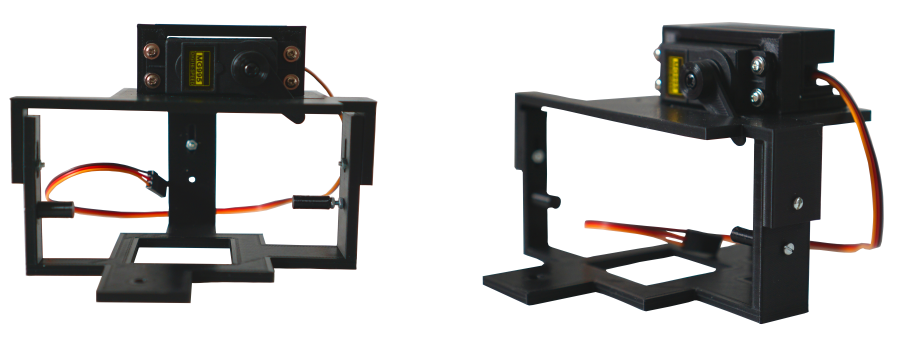
\includegraphics[width=.6\textwidth]{servoTestStation}
    \caption{Stützstruktur für einen Versuchsaufbau zum Betätigen eines Fernsteuerungstasters mittels eines Servos}
    \label{fig:servoTestStation}
\end{figure}

Für den finalen Versuchsaufbau wird als Grundlage, das Versuchsverfahren aus der Arbeit in Quelle \cite{wimmerLatenzStation} verwendet. Dieses Verfahren setzt jedoch vorraus, dass Veränderungen an der Multikopterfernsteuerung durchgeführt werden. Die Betätigung des Tasters der Fernsteuerung findet hierbei mittels eines Optokopplers statt, wodurch an dem Fernsteuerungstaster zwei Kabel angelötet werden müssen.

Ein Optokoppler ist ein Elektronikkompente mit welcher Signale galvanisch getrennt übertragen werden können \cite{elektronikKompendiumOptokoppler}. Das zu übertragende Signal wird dabei mittels einer \ac{LED} -- als Sendeelement -- und einer Fotodiode -- als Empfangselement -- übertragen, wodurch beide Teilschaltungen galvanisch getrennt sein können. Zu sehen ist das zugehörige Ersatzschaltbild eines Optokopplers in Abbildung \ref{fig:optocoupler}.

\begin{figure}[H]
    \centering
    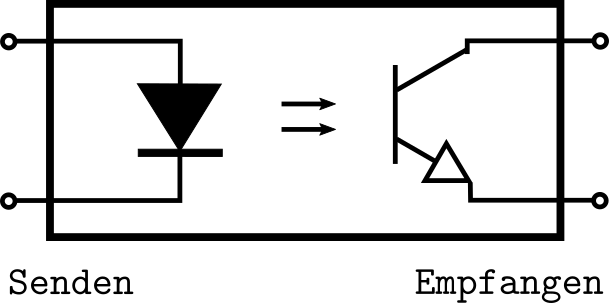
\includegraphics[width=.3\textwidth]{optocoupler}
    \caption{Ersatzschaltbild eines Optokopplers; abgewandelt von \cite{altiumOptokoppler}}
    \label{fig:optocoupler}
\end{figure}

Für die Ausführung der Latenzmesssoftware wird der Einplatinencomputer Raspberry Pi Model B+ verwendet. Dieser bietet ansteuerbare \acs{GPIO}, womit die \ac{LED} des Optokopllers geschalten wird. Betrieben wird der Einplatinencomputer mit dem Betriebssystem \textit{Raspbian GNU/Linux 11 (bullseye)} und dem Linux-Kernel Version \textit{5.15.61+}. Zur Auswertung der Eingabeereignisse im Linux-Kernel wird die Schnittstelle evdev, welche in Kapitel \ref{section:evdevExplained} beschrieben ist, verwendet. evdev kann sowohl für die Auswertung von \ac{BLE}- als auch USB-Eingabeereignisse verwendet werden. Als Latenz in diesem Versuchsaufbau wird die Zeit zwischen dem Deaktivieren der \ac{LED} des Optokopplers und dem Auftreten des Eingabeereignisses im Kernel des Einplatinencomputers verwendet. Der zugehörige Versuchsschaltplan ist in Abbildung \ref{fig:optoTestStation} zu sehen.

\begin{figure}[H]
    \centering
    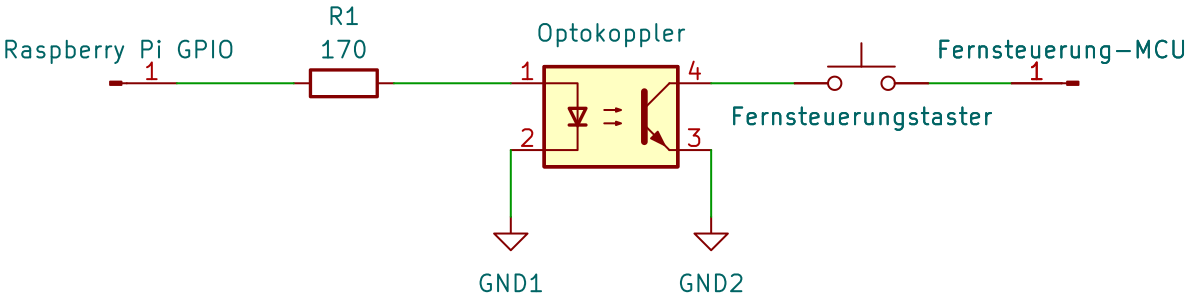
\includegraphics[width=.8\textwidth]{optoTestStation}
    \caption{Schaltplan des Versuchsaufbaus zur bestimmung der Latenz mittels eines Optokopplers; abgewandelt von \cites{wimmerLatenzStation}[S.~8; S.~12]{LTV817}}
    \label{fig:optoTestStation}
\end{figure}

\subsection{Auswertung}
Sowohl für die Auswertung der USB-Latenz als auch für die Auswertung der \ac{BLE}-Latenz erfolgten jeweils 5000 Versuchsdurchläufe. Die Versuchsergebnisse werden dabei als Schwarmplot dargestellt, indem jede Messung als eigenständiger Punkt dargestellt wird \cite[S.~7]{wimmerLatenzStation}. Dadurch können die Versuchsergebnisse dieser Arbeit gut mit den Ergebnissen aus Quelle \cite{wimmerLatenzStation} verglichen werden, da dort die Ergebnisse im selben Format bereitgestellt werden. 

\subsubsection{USB-Latenz}
In Abbildung \ref{fig:latencyUSBAll} sind alle 5000 Durchläufe des Versuchsdurchlaufs als Schwarmplot dargestellt. Während des Versuchsdurchlaufs wurden alle 5000 Tastenbefehle an der Fernsteuerung durch den Einplatinencomputer als Eingabeereigniss erkannt. Der Latenzmittelwert aller Durchläufe liegt bei 9,16~ms und die Standardabweichung bei 2,26~ms. Durch diese Ergebnisse befindet sich die Latenz mittels der USB-Verbindung der Multikopterfernsteuerung im Vergleich zu den getesten Eingabegeräten von Quelle \cite{wimmerLatenzStation} zu den 50~\% mit einer geringeren Latenz.

\begin{figure}[H]
    \centering
    \includegraphics[width=.7\textwidth]{latencyUSBAll}
    \caption{Latenz aller Versuchsdurchläufe mittels USB-Verbindung}
    \label{fig:latencyUSBAll}
\end{figure}

\subsubsection{\ac{BLE}-Latenz}
Von allen 5000 Versuchsdurchläufen mittels der \ac{BLE}-Verbindung konnten am Einplatinencomputer sieben Eingabeereignisse nicht erkannt werden. Von allen erkannten Durchläufen lag dabei der Latenzmittelwert bei 52,22~ms und die Standardabweichung bei 97,32~ms. Die Standardabweichung hat dabei einen großen Wert, da wie in Abbildung \ref{fig:latencyBLEAll} zu sehen ist 267 Messergebnisse außerhalb von 100~ms liegen und dadurch der Versuchsergebnissbereich eine große Spreizung aufweist. Werden jedoch die Messergebnisse größer 100~ms herausgerechnet liegt der Latenzmittelwert bei 30,00~ms und die Standardabweichung bei 7,68~ms, wie in Abbildung \ref{fig:latencyBLElt100} zu sehen ist. In nachfolgenden Kapitel ist beschrieben, warum Messergebnisse größer 100~ms in der Praxis vernachlässigt werden können. Jedoch gehört in beiden Fällen die \ac{BLE}-Verbindung des Fernsteuerungserweiterungsmodul zu den Eingabegeräten der Quelle \cite{wimmerLatenzStation} zu einen der langsamsten Eingabegeräten.

\begin{figure}[H]
    \centering
    \includegraphics[width=.7\textwidth]{latencyBLEAll}
    \caption{Latenz aller Versuchsdurchläufe mittels \ac{BLE}-Verbindung}
    \label{fig:latencyBLEAll}
\end{figure}

\begin{figure}[H]
    \centering
    \includegraphics[width=.7\textwidth]{latencyBLElt100}
    \caption{Latenz aller Versuchsdurchläufe die kleiner 100~ms sind mittels \ac{BLE}-Verbindung}
    \label{fig:latencyBLElt100}
\end{figure}

\subsubsection{Ergebnisse}
%Ergebnisse erläutern
%Berechnen was für eine Strecke geflogen wird in 30ms. Geschwindigkeit von Renndrohnen und normalen drohnen ausrechnen. Dabei jedoch schreiben, dass es in relation gesehen werden muss, dass pro neuen Signal nur immer von relativen Anpassungen der Flugbahn ausgegangen werden muss und nicht von 
%Auch noch schreiben, dass die Testperson (ein Hobbiedrohnenpilot) keinen merkbaren unterschied zwischen einer USB-Verbindung und BLE-Verbindung ausmachen konnte im Simulator.
%Schreiben wieso diese zusätzliche Latenz zu stande kommt und die ausreißer.
    %-nicht jedes CRSF für die Tastenstellungen
    %-Übertragungsrate von BLE
    %-Doppelte Umwandlung in verschiedene Protokolle
%auch sollten die einzelnen ausgefallenen Pakete oder die nach 100ms nicht all zu fehlerbehaftet gesehen werden, da sich ständig werte ändern während der flug einer drohne und nicht nur ein einziges signal sich ändert wodurch viel häufiger die alle Controller-Daten an das Endgerät gesendet werden
%schreiben wieso es so spikes an gewissen stellen gibt
    %-Ist von der Pollingrate von BLE und USB abhängig
% schreiben, warum man die Messergebnisse im Bereich > 100ms vernachlässigen kann